%%%%%%%%%%%%%%%%%%%%%%%%%%%%%%%%%%%%%%%%%%%%%%%%%%%%%%%%%%%%%%%%%%%%%%%%%%%%%%
%
% Section file included in main project file using \input{}
%
% Assumes that LaTeX2e macros and packages defined in cg_comp.sty are
%   available
%
%%%%%%%%%%%%%%%%%%%%%%%%%%%%%%%%%%%%%%%%%%%%%%%%%%%%%%%%%%%%%%%%%%%%%%%%%%%%%%

 \section{Experimental Estimate of the String Constant\label{sct:exp}}

How do we determine the spring constant $\kappa$ given by \eqn{kappa_def}? Ideally, we could conduct an experiment that measures the change in the frequency of an open string --- pinned at one end, and clamped at the other --- as we make slight changes to its length~\cite{ref:byers1996cgi,ref:varieschi2010icf}. From \eqn{f_m_stiff}, the derivative of the fundamental frequency of an open string is
 \begin{equation}
 \begin{split}
\frac{d\, f}{d\, L} &= \frac{f}{L} \left( -1 + \frac{L}{2\, T}\, \frac{d\, T}{d\, L} - \frac{L}{2\, \mu}\, \frac{d\, \mu}{d\, L} + \frac{L}{1 + B}\, \frac{d\, B}{d\, L} \right) \\
&= \frac{f}{L} \left( -1 + \half\, \kappa + \half - \frac{B}{1 + B} \right) \\
&\approx \frac{f}{L} \times \half\, (\kappa - 1)\, ,
 \end{split}
 \end{equation}
where we have used the analysis in \sct{model} to determine that
 \begin{subequations}
 \begin{align}
\frac{d\, T}{d\, L} &= \frac{T}{L}\, \kappa\, , \\
\frac{d\, \mu}{d\, L} &= -\frac{\mu}{L}\, , \nd \\
\frac{d\, B}{d\, L} &= -\frac{B}{L}\, . \\
 \end{align}
 \end{subequations}
Therefore, following Byers~\cite{ref:byers1996cgi,ref:varieschi2010icf}, we define the parameter $R$ to be
 \begin{equation}\label{eqn:r_def}
R \equiv \frac{L}{f}\, \frac{d\, f}{d\, L} = \half\, (\kappa - 1)\, ,
 \end{equation}
which gives
 \begin{equation} \label{eqn:kappa_r}
\kappa = 2\, R + 1\, .
 \end{equation}
With this measurement of $\kappa$, we can estimate the bending stiffness coefficient by comparing \eqn{kappa_def} and \eqn{bg_n_def}, and writing $B_0$ as
 \begin{equation} \label{eqn:b_0_kappa}
B_0 = \sqrt{\kappa}\, \frac{\rho}{2\, L_0}\, .
 \end{equation}

It is relatively easy to estimate the values of $\kappa$ and $R$ for any guitar string with the aid of a simple device that can measure frequency shifts in cents~\cite{ref:pgtweb}. First, we tune the open string to the correct 12-TET frequency. Then, we select a fret $n$, and measure the frequency deviation $\Delta \nu_n$ of the fretted string. If we substitute \eqn{b_0_kappa} into \eqn{error_tot}, then we find
 \begin{equation} \label{eqn:root_kappa_quad}
\alpha\, \kappa + \beta\, \sqrt{\kappa} - \xi = 0\, ,
 \end{equation}
where we have included the quadratic bending stiffness term, and defined the coefficients
 \begin{subequations}
 \begin{align}
\alpha &\equiv \half \left[ Q_n + \left(\gamma_n^2 - 1\right)\left(1 + \pi^2\right)\left(\frac{\rho}{2\, L_0}\right)^2 \right]\, , \\
\beta &\equiv \left(\gamma_n - 1\right)\, \frac{\rho}{2\, L_0}\, , \nd \\
\xi &\equiv \frac{\ln(2)}{1200}\, \Delta \nu_n + \frac{\left(\gamma_n - 1\right) \Delta S - \Delta N}{X_0}\, .
 \end{align}
 \end{subequations}
\Eqn{root_kappa_quad} is quadratic in $\sqrt{\kappa}$, with the solution
 \begin{equation} \label{eqn:root_kappa_soln}
\sqrt{\kappa} = \frac{-\beta + \sqrt{\beta^2 + 4\, \alpha\, \xi}}{2\, \alpha}\, ,
 \end{equation}
where we have chosen the positive root.

We've used this approach to estimate $\kappa$ and $R$ of different string sets on the Alhambra 8P classical guitar, which has $X_0 = 650$~mm, $c = 3.5$~mm, $\Delta S = 1.5$~mm, and $\Delta N = 0.0$~mm. At the nut, $b = 1.0$~mm, but the height of the fret board decreases roughly linearly further toward the saddle, effectively increasing $b$. We estimate that $d b / d x \approx -0.0034$, so that $b$ has increased to 2.0~mm at the 12$^{\text{th}}$ fret. We show the specifications of a normal-tension classical string set in \tbl{ej45_mks} using metric units\footnote{Note that the correct unit of force in the metric system is Newtons (N), rather than kilograms, which is a unit of mass.}. In \tbl{ej45_props}, we list the frequency deviation from 12-TET at the 12$^{\text{th}}$ fret for each string in this set, as well as the corresponding estimates of $\kappa$, $R$, $E$, and $B_0$, computed from \eqn{root_kappa_soln}, \eqn{r_def}, \eqn{kappa_def}, and \eqn{b_0_kappa}, respectively. The units used for the elastic modulus are gigapascals (1 GPa = $10^9$~N/m$^2$.). Similar measurements and results for other string sets are provided in \app{specs}.


%Recall how we introduced this concept in \sct{model_tension}: increasing the tension by a quantity $\Delta T$ causes a shift in the frequency of a guitar string by $\Delta \nu$ in cents. Although we were considering fretted strings when we derived \eqn{error_def}, the terms in that equation can be generalized to describe the case of an open string that has been stretched longitudinally. Suppose that we continue to clamp the string at the saddle and the nut, but that we tighten the tuning gear to stretch that string's length by an amount $\Delta L$. The change in the string's frequency due to the change in the open resonant length is zero, because $L_0 / \gamma_0 L_0 = 1$. The linear mass density of the string is smaller now because there is less material between the saddle and the nut, causing the frequency shift (in cents)
% \begin{equation}
%600\, \log_2 \left(  \frac{\mu}{\mu + \Delta \mu} \right) \approx \frac{600}{\ln(2)}\, \frac{\Delta L}{L}\, ,
% \end{equation}
%where $L$ is the initial length of the string. Finally, the tension in the string increases by $\Delta T$ due to the elastic properties of the string. Following the discussion in \sct{model_tension}, the corresponding frequency shift  is
% \begin{equation}
%600\, \log_2 \left(  \frac{T + \Delta T}{T} \right) \approx \frac{600}{\ln(2)}\, \frac{\Delta L}{L}\, \kappa\, ,
% \end{equation}
%where $T$ is the initial tension of the string. Therefore, the total frequency shift of the open string caused by a change $\Delta L$ in the string's length is
% \begin{equation}
%\Delta \nu \approx \frac{600}{\ln(2)}\, \frac{\Delta L}{L}\, (\kappa + 1)\, ,
% \end{equation}
%characterizing the string frequency's response to a change in length. It is dominated by the change in the tension of the string, and given $R$ we can quickly determine $\kappa$.
%
%
%Solving this expression for the string constant, we find
% \begin{equation}
%\kappa = \frac{\ln(2)}{600}\, R - 1\, ,
% \end{equation}
%where
% \begin{equation}
%R \equiv \frac{L}{\Delta L}\, \Delta \nu
% \end{equation}
%is a parameter originally defined by Byers\footnote{Byers expressed this parameter in terms of the fractional frequency shift (in Hertz) as $R = (L/\Delta L) (\Delta f/f) \approx (\ln(2)/1200) (L/\Delta L) \Delta \nu$. Therefore, our dimensionless value of $R$ is larger than Byers' by a factor of about 1730.}~\cite{ref:byers1996cgi,ref:varieschi2010icf}.

% \begin{equation}
% \begin{split}
%L_{n \ge 1}(y) &= \sqrt{\left(X_n + \Delta S\right)^2 + (b + c)^2 + y^2} \\
%&\approx X_n + \Delta S + \frac{(b + c)^2 + y^2}{2\, X_n}\, .
% \end{split}
% \end{equation}
%
% \begin{equation}
% \begin{split}
%L^\prime_{n \ge 1}(y) &= \sqrt{\left(X_0 - X_n + \Delta N\right)^2 + b^2 + y^2} \\
%&\approx X_0 - X_n + \Delta N + \frac{b^2 + y^2}{2 \left(X_0 - X_n\right)}\, .
% \end{split}
% \end{equation}
%
% \begin{equation}
% \begin{split}
%Q_n(y) &\approx \frac{1}{2\, X_0} \left[ \frac{(b + c)^2 + y^2}{X_n} + \frac{b^2 + y^2}{X_0 - X_n} - \frac{c^2}{X_0} \right] \\
%&= Q_n(0) + \Delta Q_n(y) \, ,
% \end{split}
% \end{equation}
%where $Q_n(0)$ is given by \eqn{lambda_n_approx}, and
% \begin{equation}
%\Delta Q_n(y) \equiv \frac{1}{2 \left(\gamma_n - 1\right)}\, \left(\frac{\gamma_n\, y}{X_0}\right)^2\, .
% \end{equation}
%
%Following the same approach we used to derive \eqn{quad_shift}, we can derive the change in the total shift due to both resonant length and linear mass density for a transverse displacement $y$. To second order in $y$, we find that
% \begin{equation}
%\Delta \nu_n(y) \approx \frac{600}{\ln(2)}\, \frac{3 - 2 \gamma_n}{2 \left(\gamma_n - 1\right)}\, \left(\frac{\gamma_n\, y}{X_0}\right)^2\, .
% \end{equation}
%We have plotted this expression for the first 12 frets and $y = 5$~mm in \fig{quad_shift_factory}. This shift is quite small compared to the experimental errors we'll obtain in the shifts due to tension, and we ignore it in what follows.
%
% \begin{figure}
%  \centering
%  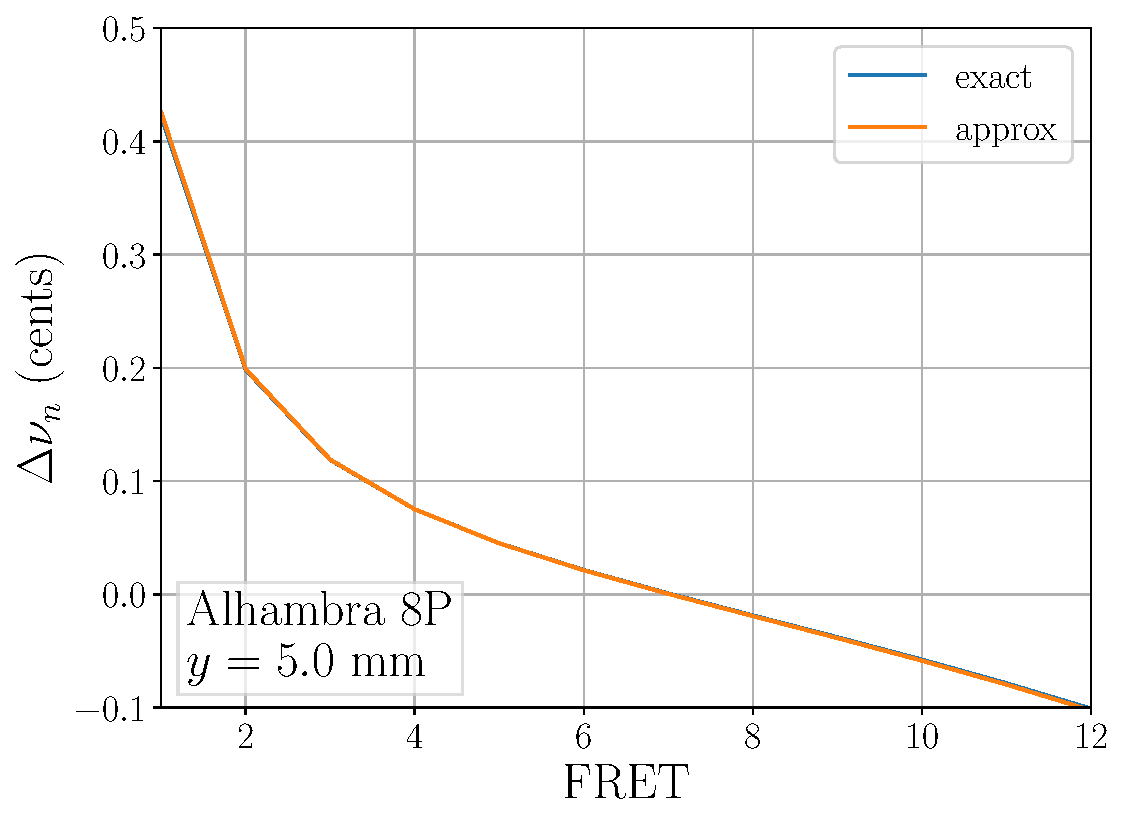
\includegraphics[width=5.0in]{figures/quad_shift_factory}
%  \caption{\label{fig:quad_shift_factory} Total frequency shift (in cents) due to resonant length and linear mass density for a transverse displacement of $y = 5$~mm. This shift is identical for each string, and should be smaller than the experimental errors we'll accumulate using our transverse displacement approach.}
% \end{figure}
%
%\begin{table}%[htbp]
%  \centering
%  \caption{\label{tbl:ej43_props} Derived physical properties of the D'Addario Pro-Arte Nylon Classical Guitar Strings -- Light Tension (EJ43). The corresponding scale length is 650 mm.}
%    \begin{tabular}{lcccc}
%    \hline \hline
%    String  & $R$ & $\kappa$ & Modulus (GPa) & Stiffness \\
%    \hline
%    J4301 & 4.39 $\times 10^{4}$ & 49.8 & 8.62 & 3.79 $\times 10^{-3}$ \\
%    J4302 & 5.02 $\times 10^{4}$ & 57.0 & 5.62 & 4.68 $\times 10^{-3}$ \\
%    J4303 & 4.79 $\times 10^{4}$ & 54.4 & 3.57 & 5.72 $\times 10^{-3}$ \\
%    J4304 & 5.02 $\times 10^{4}$ & 57.0 & 9.52 & 4.13 $\times 10^{-3}$ \\
%    J4305 & 4.39 $\times 10^{4}$ & 49.8 & 5.05 & 4.55 $\times 10^{-3}$ \\
%    J4306 & 5.27 $\times 10^{4}$ & 59.9 & 3.97 & 6.35 $\times 10^{-3}$ \\
%    \hline
%    \end{tabular}%
%  \label{tab:addlabel}%
%\end{table}%

%\begin{table}[htbp]
%  \centering
%  \caption{\label{tbl:ej45_ips} String specifications for the D'Addario Pro-Arte Nylon Classical Guitar Strings -- Normal Tension (EJ45). The corresponding scale length is 25.5~inches.}
%    \begin{tabular}{lcccc}
%    \toprule
%    String  & Note  & \multicolumn{1}{l}{Diameter (in)} & \multicolumn{1}{l}{Density (lb/in)} & \multicolumn{1}{l}{Tension (lb)} \\
%    \midrule
%    J4501 & $E_4$  & 0.0280 & $2.092 \times 10^{-5}$ & 15.3 \\
%    J4502 & $B_3$  & 0.0322 & $2.827 \times 10^{-5}$ & 11.6 \\
%    J4503 & $G_3$  & 0.0403 & $4.679 \times 10^{-5}$ & 12.1 \\
%    J4504 & $D_3$  & 0.0290 & $1.075 \times 10^{-4}$ & 15.6 \\
%    J4505 & $A_2$  & 0.0350 & $1.842 \times 10^{-4}$ & 15.0 \\
%    J4506 & $E_2$  & 0.0430 & $3.063 \times 10^{-4}$ & 14.0 \\
%    \bottomrule
%    \end{tabular}%
%\end{table}%

\begin{table}[htbp]
  \centering
  \caption{\label{tbl:ej45_mks} String specifications for the D'Addario Pro-Arte Nylon Classical Guitar Strings -- Normal Tension (EJ45). The corresponding scale length is 650~mm.}
  \begin{tabular}{cccccc}
\toprule
String & Note & Radius (mm) & Density ($\times 10^{-7}$ kg/mm) & Tension (N) \\
\midrule
J4501 & E$_{4}$ & 0.356 & 3.74 & 68.6 \\
J4502 & B$_{3}$ & 0.409 & 5.05 & 52.0 \\
J4503 & G$_{3}$ & 0.512 & 8.36 & 54.3 \\
J4504 & D$_{3}$ & 0.368 & 19.21 & 70.0 \\
J4505 & A$_{2}$ & 0.445 & 32.90 & 67.3 \\
J4506 & E$_{2}$ & 0.546 & 54.72 & 62.8 \\
\bottomrule
\end{tabular}


\end{table}%

\begin{table}[htbp]
  \centering
  \caption{\label{tbl:ej45_props} Derived physical properties of the D'Addario Pro-Arte Nylon Classical Guitar Strings -- Normal Tension (EJ45). The corresponding scale length is 650 mm.}
  \begin{tabular}{cccccc}
\toprule
String & $R$ & $\sigma$ & $\kappa$ & $B_0$ & $E$ (GPa) \\
\midrule
J4501 & 23.6 & 0.5 & 48.2 & 0.00190 & 8.33 \\
J4502 & 23.8 & 0.7 & 48.6 & 0.00219 & 4.81 \\
J4503 & 28.8 & 0.7 & 58.7 & 0.00302 & 3.87 \\
J4504 & 22.4 & 0.8 & 45.7 & 0.00192 & 7.51 \\
J4505 & 23.8 & 0.8 & 48.6 & 0.00238 & 5.27 \\
J4506 & 28.6 & 0.4 & 58.2 & 0.00321 & 3.90 \\
\bottomrule
\end{tabular}


\end{table}%

